% Вторая глава работы 
\chapter{Обзор дисциплины управлением очередью RED}
\label{chap2}

В данном разделе представим описание работы нескольких алгоритмов семейства RED и их реализацию в NS-2 и mininet. 


\section{Классическая модификация}
\label{chap2:sec1}

Random Early Detection (RED) — это семейство механизмов предотвращения перегрузки
на шлюзе. Он основан на общих принципах, полезен для управления
средним размером очереди в сети, где не доверяют взаимодействию между
протоколами передачи данных. В отличие от Droptail, который работает
таким образом, что когда очередь заполняется, новые пакеты,
поступающие в очередь, начинают теряться, алгоритм RED учитывает
потоки трафика в сети и стремится предоставить равную пропускную
способность для каждого соединения, что позволяет избежать перегрузки
сети и улучшить качество обслуживания. В оригинальном RED
маршрутизатор вычисляет усредненный по времени средний размер очереди
с использованием фильтра нижних частот (экспоненциально взвешенное
скользящее среднее) или сглаживания по длине выборки очередей, средний
размер очереди сравнивается с двумя пороговыми значениями: минимальным
порогом и максимальным. Когда средний размер очереди меньше
минимального порога, пакеты не отбрасываются, когда средний размер
очереди превышает максимальный порог, отбрасывается все поступающие
пакеты. Если размер средней очереди находится между минимальным и
максимальным порогом, пакеты отбрасываются с вероятностью $p$, которая
линейно увеличивается до тех пор, пока средняя очередь не достигнет
максимального порога. Подробно классический алгоритм описан в~\cite{RED1, RED0}.


На рисунке ~\ref{fig1} представлена вероятная функция сброса пакетов.
 
\begin{figure}[h!]
 \centerline{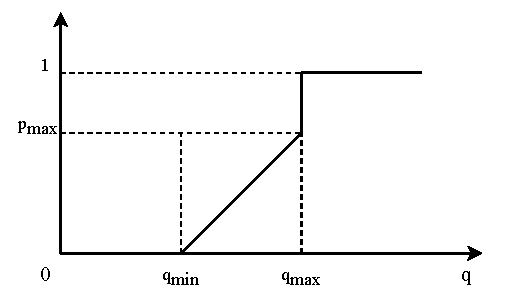
\includegraphics[width=0.7\textwidth]{red_plot}}
 \caption{Вид функции сброса в алгоритме RED}
\label{fig1}
\end{figure}


Вероятность $p_{b}$ маркировки на отбрасывание пакетов представляет
собой функцию, линейно зависящую от $\hat{q}$ (средневзвешенное
скользящее среднее), минимального $q_{\min}$ и максимального
$q_{\max}$ пороговых значений и параметра $p_{\max}$, определяющего
часть отбрасываемых пакетов при достижении средним размером очереди
значения $q_{\max}$ и вычисляется следующим образом \eqref{eq2:1}:

\begin{equation}
\label{eq2:1}
p_{b} = \begin{cases}
        0, &  \ 0 < \hat{q} \leqslant q_{\min},
        \\
        \frac{\hat{q} - q_{\min}}{q_{\max} - q_{\min}} p_{\max}, & \ q_{\min} < \hat{q} \leqslant q_{\max}, 
        \\
        1, &  \ \hat{q} > q_{\max}.
\end{cases}                                     
\end{equation}


В NS-2 файлы, связанные с RED, прописаны в каталоге
\verb|ns-2.35/queue|, там представлены также другие реализации
очередей (среди них DropTail, BLUE и т.д.). Следует уделить внимание
двум файлам: \verb|red.cc| (исходники), и \verb|red.h| (заголовочный
файл). Вероятность отбрасывания пакета прописана в функции

\verb|double REDQueue::calculate_p_ne файла red.cc|

Для реализации в NS-2 необходимо указать в качестве очередей между соединениями
RED, и при настройке очереди указать минимальные и максимальные пороговые значения 
\verb|(thresh_ и maxthresh_)|, величина, обратное параметру максимального сброса\verb|(linterm_)|, 
а также указать параметр \verb|gentle_| false.

Для реализации в Mininet используем утилиту tc qdisk ... red, имеющий следующие опции:
\begin{itemize}
\item min: минимальный порог, по достижении которого возникает вероятность отметки пакета.
\item max: максимальный порог очереди
\item probability: максимальная вероятность пометки, указанная как число с плавающей точкой, от 0.0 до 1.0. 
\item limit: жесткий предел реального (не среднего) размера очереди в байтах. По достижении этого размера все лишние пакеты будут отброшены.
\item burst: используется для определения того, как реальный размер очереди начинает влиять на средний размер очереди. 
\item avpkt: указывается в байтах. Используется вместе с burst для определения временной константы для вычисления среднего размера очереди. 1000 - неплохое значение.
\item bandwidth: используется для расчета среднего размера очереди после простоя в течение некоторого времени. Должно быть равным значению пропускной способности интерфейса. Не влияет на параметр пропускной скорости интерфейса. Необязательное значение.

\end{itemize}

Существует несколько причин, по которым существует множество вариаций алгоритмов семейства RED:

\begin{enumerate}
\item Разнообразные сетевые сценарии: Разные сетевые сценарии требуют разных настроек и параметров для эффективного управления потоком. Например, алгоритм RED может быть настроен по-разному для использования в локальной сети (LAN) и в глобальной сети (WAN) или в сетях с разной пропускной способностью.
\item Разные типы сетей: RED может быть применен в разных типах сетей, включая проводные и беспроводные сети, и разные типы сетей могут иметь уникальные характеристики и требования, которые влияют на алгоритм.
\item Эволюция сетевых технологий: Сетевые технологии постоянно развиваются, и новые требования и возможности могут потребовать адаптации алгоритма RED. Например, изменения в сетевых протоколах или появление новых типов трафика могут потребовать модификаций алгоритма RED.
\item Эксперименты и исследования: Сетевые исследователи могут создавать различные вариации RED для проведения экспериментов и оценки их производительности в различных условиях.
\item Открытая архитектура: RED - это открытая архитектура, что позволяет исследователям и инженерам создавать свои собственные модификации и адаптации алгоритма в соответствии с конкретными потребностями и задачами.
\end{enumerate}


\section{Нелинейные модификации}
\label{chap2:sec2}

Nonlinear RED~--- это модификация классического алгоритма RED, в
котором используется нелинейная функция для определения
вероятности отбрасывания пакетов. Nonlinear RED предназначен для более точной адаптации к изменениям трафика и динамике сети. 
Он способен эффективно реагировать на изменения величины очереди и адаптироваться к различным условиям сети. 
Это позволяет более гибко управлять задержкой пакетов и предотвращать перегрузки в сети, 
что делает Nonlinear RED более эффективным по сравнению с классическим алгоритмом RED.~\cite{NLRED1, NLRED2}.   


Вероятность $p_{b}$ маркировки на
отбрасывание пакетов вычисляется следующим способом \eqref{nlred}:

\begin{equation}
\label{nlred}
p_{b} = \begin{cases}
        0, &  \ 0 < \hat{q} \leqslant q_{\min},
        \\
        1.5({\frac{\hat{q} - q_{\min}}{q_{\max} - q_{\min}})^2} {p_{\max}}, & \ q_{\min} < \hat{q} \leqslant q_{\max},
        \\
        1, &  \ \hat{q} > q_{\max}.
\end{cases}
\end{equation}


По умолчанию NLRED не реализован в NS-2. Для её добавления я использовал патч для данной модификации, созданный Mohit
  P. Tahiliani для версии 2.34, совместимой также для версии 2.35 ~\cite{nlredpatch}. 
  
\begin{enumerate}
\item Установил к себе на машину патч \verb|NLRED.patch| от 
\item Отредактировал файл, заменив везде номер версии на 2.35 и переместил в каталог \verb|ns-allinone|.
\item Дополнил файлы \verb|queue/red.cc|, \verb|queue/red.h|, \verb|tcl/ns-default.tcl| строками из патча, .
\item Переустановил программу.
\item В настройке очереди сети указал значение переменной \verb|nonlinear_ 1|.
\end{enumerate}



GRED (Gentle Random Early Detection, мягкое/аккуратное произвольное
раннее обнаружение)~--- алгоритм активного управления очередью,
является расширением RED. Стандартный алгоритм увеличивает
вероятность отбрасывания с 0.05 до 0.5, когда средняя длина очереди
увеличивается от минимального до максимального порогового значения, но
при превышении максимального порога вероятность возрастает напрямую с
0.5 до 1.  Этот внезапный скачок нормализуется модификацией Gentle
RED, который расширяет RED тем, что добавляет дополнительное
максимальное пороговое значние, которое равно $2q_{\max}$, тем самым
<<сглаживая>> кривую~\cite{GRED}. Однако, например, задача минимального порога в данной модификации не меняется, 
и увеличение лишь максимального порога для отбрасывания всех пакетов делает GRED лишь частным случаем классического алгоритма. 
Данная модификация в NS-2 используется по умолчанию, так как переменная \verb|gentle_| по умолчанию 
является истинной. 

Вероятность сброса определяется по формуле \eqref{gred}:

\begin{equation}
\label{gred}
p_{b} =\begin{cases}
        0, &  \  0 < \hat{q} \leqslant q_{\min}, 
        \\
        \frac{\hat{q} - q_{\min}}{q_{\max} - q_{\min}} p_{\max}, & \ q_{\min} \leqslant \hat{q} < q_{\max}, 
        \\
        \frac{\hat{q} - q_{\min}}{q_{\max}}(1-p_{\max}) - p_{\max}, & \ q_{\max} \leqslant \hat{q} < 2q_{\max}, 
        \\
        1, &  \ \hat{q} \geqslant  q_{\max}.
\end{cases}
\end{equation}


WRED (Weighted random early detection --- взвешенное произвольное раннее
обнаружение)~--- это алгоритм активного управления очередью, является
расширением RED~\cite{WRED}.

Взвешенный алгоритм произвольного раннего обнаружения предоставляет
различные уровни обслуживания пакетов в зависимости от вероятности их
отбрасывания и обеспечивает избирательную установку параметров
механизма RED на основании типа трафика.

Алгоритм DS-RED(Double slope random early detection)~--- это ещё одна модификация RED, в котором вводится дополнительное пороговое значение $q_{mid}$ между минимальным $q_{min}$ и максимальным
REDФункция сброса описывается двумя линейными сегментами с углами наклона $\alpha $ и $\beta $ соответственно, регулируемыми
задаваемым селектором режимов $\gamma$ ~\cite{DSRED}.  По умолчанию модификация не реализована в NS-2, для её реализации дополнил фунцию \verb|double REDQueue::calculate_p_ne файла red.cc|, а в программе очереди указал значение переменной \verb|double_slope_ 1|. 

Функция вероятности сброса пакетов в алгоритме DSRED показана в формуле \eqref{dsred}

\begin{equation}
\label{dsred}
p_{b} =\begin{cases}
        0, &  \  0 < \hat{q} \leqslant q_{min}, 
        \\
        \alpha{\hat{q} - q_{min}}, & \ q_{min} \leqslant \hat{q} < q_{mid}, 
        \\
        1 - \gamma + \beta{\hat{q} - q_{mid}}, & \ q_{mid} \leqslant \hat{q} < q_{max}, 
        \\
        1, &  \ \hat{q} \geqslant  q_{max}.
\end{cases}
\end{equation}

где $\alpha = (\frac{2(1 - \gamma)}{\hat{q} - q_{\min}})$, а $\beta = (\frac{2\gamma}{\hat{q} - q_{min}})$


HRED(Hyperbola random early detection) ~---это модификация классического RED с нилейно возрастающей функцией отбрасывания пакетов в сети.
HRED менее чувствителен к настройкам параметров, чем другие схемы. При заданном значении $q_{\max}$ HRED ведет себя похожим образом и не сильно зависит от других параметров.
HRED может достичь более высокого использования сети. HRED обеспечивает предсказуемую задержку в очереди сети. HRED сохраняет способность контролировать кратковременную перегрузку путем поглощения пакетных потоков, так как он все еще использует алгоритм подсчета среднего размера очереди и поддерживает неполную очередь. Размер очереди может быть задан и зависит от требований. HRED прост в реализации и легко внедряется на маршрутизаторах, так как зменяется только профиль отбрасывания по сравнению с классическим алгоритмом RED~\cite{HRED}. По умолчанию модификация не реализована в NS-2, для её реализации дополнил фунцию \verb|double REDQueue::calculate_p_ne файла red.cc|, а в программе очереди указал значение переменной \verb|hyperbola_ 1|.
 
Вероятность $p_{b}$ маркировки на
отбрасывание пакетов вычисляется следующим способом \eqref{hred}:

\begin{equation}
\label{hred}
p_{b} = \begin{cases}
        0, &  \ 0 < \hat{q} \leqslant q_{\min},
        \\
        1.5({\frac{\hat{q} - q_{\min}}{q_{\max} - q_{\min}})^{-1}} {p_{\max}}, & \ q_{\min} < \hat{q} \leqslant q_{\max},
        \\
        1, &  \ \hat{q} > q_{\max}.
\end{cases}
\end{equation}


TRED(Three-section random early detection) ~--- это разновидность алгоритма RED, основанный на Nonlinear RED, которая направлена на решение проблем недостаточного использования пропускной способности и больших задержек, возникающих при низкой и высокой нагрузке в RED. 
Средняя длина очереди TRED между двумя пороговыми значениями разделена на три равные секции, и вероятность отбрасывания пакетов для каждой секции устанавливается по-разному, чтобы адаптироваться к различным трафиковым нагрузкам. С использованием симуляции в среде NS2, TRED эффективно устраняет недостатки RED, увеличивая пропускную способность при низкой нагрузке и снижая задержку при высокой нагрузке. TRED улучшает способность регулировать сетевую перегрузку, повышая использование ресурсов сети и стабильность схемы. В дальнейших исследованиях мы заинтересованы в изучении TRED с явным уведомлением о перегрузке (ECN), поскольку множество исследований показало, что AQM с ECN работает более эффективно, чем без ECN.~\cite{TRED}. По умолчанию модификация не реализована в NS-2, для её реализации дополнил фунцию \verb|double REDQueue::calculate_p_ne файла red.cc|, а в программе очереди указал значение переменной \verb|three_sections_ 1|. 

Вероятность $p_{b}$ маркировки на отбрасывание приведена в \eqref{TRED}, где $ \delta = (q_{max} - q_{min})/3 $.

\begin{equation}
\label{TRED}
p_{b} = \begin{cases}
        0, &  \ 0 \leqslant \hat{q} < q_{\min},
        \\
        9({\frac{\hat{q} - q_{\min}}{q_{\max} - q_{\min}})^3} {p_{\max}}, & \ q_{\min} \leqslant  \hat{q} < q_{\min + \delta},
        \\
        (\frac{\hat{q} - q_{\min}}{q_{\max} - q_{\min}}) {p_{\max}}, & \ q_{\min} + \delta \leqslant \hat{q} < q_{\min + 2\delta},
        \\
        9({\frac{\hat{q} - q_{\min}}{q_{\max} - q_{\min}})^3} {p_{\max}} + {p_{\max}}, & \ q_{\min} +2\delta \leqslant  \hat{q} < q_{\max},
        \\
        1, &  \ \hat{q} \geqslant q_{\max}.
\end{cases}
\end{equation} 


RED-QL(Random early detection-quadratic linear) ~---модификация алгоритма RED, также является разновидностью алгоритма с нелинейно возрастающей функцией. RED-QL имеет квадратично-линейную форму и определяется на основе параметров, которые могут быть настроены для определенных требований сети\cite{REDQL} По умолчанию модификация не реализована в NS-2, для её реализации дополнил фунцию \verb|double REDQueue::calculate_p_ne файла red.cc|, а в программе очереди указал значение переменной \verb|quadratic_linear_ 1|. . 

Вероятность $p_{b}$ маркировки на отбрасывание приведена в \eqref{RED-QL}, где $ Target = 2(q_{max} + q_{min})/3 - q_{min} $.

\begin{equation}
\label{RED-QL}
p_{b} = \begin{cases}
        0, &  \ 0 \leqslant \hat{q} < q_{\min},
        \\
        9({\frac{\hat{q} - q_{min}}{2(q_{\max} - 2q_{\min}})^2} {p_{\max}}, &  q_{\min} \leqslant  \hat{q} < {Target},
        \\
        p_{max} + 3(1-p_{max}) (\frac{\hat{q} - Target}{q_{\max} + q_{\min}}), & {Target} \leqslant  \hat{q} < q_{max},
        \\
        1, &  \ \hat{q} \geqslant q_{max}.
\end{cases}
\end{equation}

\section{Адаптивные модификации}
\label{chap2:sec3}

В алгоритме Adaptive RED (ARED) функция сброса модифицируется
посредством изменения по принципу AIMD, заключающейся в том, что
увеличение некоторой величины производится путём сложения с некоторым
параметром, у уменьшение~--- путём умножения на
параметр ~\cite{ARED}. Для её реализации в NS-2 необходимо указать в
настройке очереди \verb|set adaptive_ 1|. Для реализации в Mininet нужно указать в tc дополнительно adaptive

Алгоритм ARED функционирует следующим образом (\eqref{ad1}),
(\eqref{ad2}). Для каждого интервала \verb|interval| (параметр) в
секундах, если $\hat{q}$ больше целевой (желаемой) $\hat{q_t}$ и
$p_{\max} \leqslant 0,5$, то $p_{\max}$ увеличивается на некоторую
величину $\alpha$; в противном случае, если $\hat{q}$ меньше целевой
$\hat{q_t}$ и $p_{\max}\geqslant 0,01$, то $p_{\max}$ уменьшается в
$\beta$ раз, $\alpha$ и $\beta$ задаются командами \verb|set alpha_| и \verb|set beta_|:

\begin{equation}
\label{ad1}
p_{\max} = \left\{
  \begin{aligned}
    & p_{\max}+\alpha, \ \hat{q}>\hat{q_{t}}, \ p_{\max} \leqslant 0,5, \\
    & \beta p_{\max}, \ \hat{q}<\hat{q_{t}}, \ p_{\max} \geqslant 0,01, 
  \end{aligned}
\right.
\end{equation}

\begin{equation}
\label{ad2}
q_{\min}+0,4(q_{\max}-q_{\min}) < \hat{q_t} < q_{\min}+0,6\left(q_{\max}-q_{\min}\right).
\end{equation}

Основные особенности: 
\begin{itemize}
\item автоматическая установка минимального порога $q_{\min}$. Он
  устанавливается в зависимости от пропускной способности канала $C$ и
  задержки целевой очереди, $q_{max}$ приравнивается к $3q_{min}$;
\item автоматическая настройка $w_{q}$. Он устанавливается в
  зависимости от пропускной способности канала $C$;
\item адаптивная настройка $p_{\max}$. Он адаптирован в соответствии с
  текущей средней длиной очереди;
\item рекомендованными значениями параметров являются $\alpha < 0.25 $ и $\beta > 0.83 $.
\end{itemize}


SmRED(Smart random early detection) ~--- модификация RED, в которой
вероятность отбрасывания пакетов регулируется в зависимости от нагрузки трафика для достижения оптимальной сквозной производительности.
Кроме того, переход с RED на SmRED в реальной сети требует очень мало работы из-за своей простоты. SmRED эффективно устраняет недостатки
RED, увеличивает пропускную способность при низкой нагрузке и уменьшает задержку при высокой нагрузке ~\cite{SmRED}. По умолчанию модификация не реализована в NS-2, для её реализации дополнил фунцию \verb|double REDQueue::calculate_p_ne файла red.cc|, а в программе очереди указал значение переменной \verb|smart_ 1|. 

Вероятность $p_{b}$ маркировки на отбрасывание приведена в \eqref{SmRED}, где $ Target = (q_{max} - q_{min})/2 + q_{min} $.

\begin{equation}
\label{SmRED}
p_{b} = \begin{cases}
        0, &  \ 0 \leqslant \hat{q} < q_{\min},
        \\
        ({\frac{\hat{q} - q_{min}}{q_{\max} - q_{\min}})^2} {p_{\max}}, &  q_{\min} \leqslant  \hat{q} < {Target},
        \\
        \sqrt{{\frac{\hat{q} - q_{min}}{q_{\max} - q_{\min}}}} {p_{\max}}, & {Target} \leqslant  \hat{q} < q_{max},
        \\
        1, &  \ \hat{q} \geqslant q_{max}.
\end{cases}
\end{equation}
 

Алгоритм Refined ARED предлагает более активно изменять вероятность сброса $p_{\max}$,
чтобы иметь возможность быстрой адаптации к изменяющейся
экспоненциально взвешенной скользящей средней длине очереди $\hat{q}$ ~\cite{RARED}.

Функции изменения параметра $p_{\max}$ представлена ниже(\eqref{rf1}), (\eqref{rf2}):

\begin{equation}
\label{rf1}
p_{max} = \left\{
  \begin{aligned}
& p_{\max}+\alpha, \quad  \hat{q}>\hat{q_{t}}, \quad p_{max} \leqslant 0,5, \\
& \beta p_{\max}, \quad \hat{q}\leqslant\hat{q_{t}}, \quad p_{max} > 0,5,
  \end{aligned}
\right.
\end{equation}

\begin{equation}
\label{rf2}
\left\{
  \begin{aligned}
    & q_{\min}+0,48\left(q_{\max}-q_{\min}\right) < \hat{q_t} < q_{\min}+0,52\left(q_{\max}-q_{\min}\right), \\
    & \alpha=\left(0,25\frac{\hat{q}-\hat{q_t}}{\hat{q_t}} \right)p_{\max}, \\ 
    & \beta=1-\left(0,17\frac{\hat{q}-\hat{q_t}}{\hat{q_t}-q_{\min}}\right).
  \end{aligned}
\right.
\end{equation}


По умолчанию RARED не реализован в NS-2. Для её добавления я использовал патч для данной модификации, созданный Mohit
  P. Tahiliani для версии 2.34, совместимой также для версии 2.35 ~\cite{refinedpatch}. 

\begin{enumerate}
\item Установил к себе на машину патч \verb|RARED.patch| от 
\item Отредактировал файл, заменив везде номер версии на 2.35 и переместил в каталог \verb|ns-allinone|.
\item Дополнил файлы \verb|queue/red.cc|, \verb|queue/red.h|, \verb|tcl/ns-default.tcl| строками из патча.
\item Переустановил программу.
\item В настройке очереди указал значение \verb|adaptive_ 1| и 
\verb|refined_adaptive_ 1|.
\end{enumerate}
 
 
Powared является модификацией алгоритма ARED ~\cite{Powared}. В данной модификации величина $p_{max}$ максимального сброса считается следующим образом(\eqref{powared}). Алгоритм POWARED более агрессивно реагирует на изменение cредней очереди, чем ARED. Данная модификация не реализована в NS-2, для её моделирования я в файл red.cc добавил функцию \verb|void REDQueue::updateMaxP_powared|, а в настройке очереди сети указал значение переменных \verb|adaptive_ 1| и \verb|powared_ 1|. 
Параметры модификации задаются с помощью переменных \verb|pwk_, pwb_|.

\begin{equation}
\label{powared}
p_{max} =\begin{cases}
        p_{max}-\delta_1, &  \  q_{\min} \leqslant \hat{q} < q_{mid}, 
        \\
        p_{max}+\delta_2, & \ q_{mid} < \hat{q}  \leqslant q_{max}, 
        \\
        p_{max}, &  \ \hat{q} =  q_{mid},
\end{cases}
\end{equation}

где $q_{mid} = 0.5(q_{min} + q_{max})$, 
$\delta_1 = |\frac{((\hat{q} - q_{mid})}{(\beta q_{mid}))}|^K $, а $\delta_2 = |\frac{((q_{mid} - \hat{q})}{(\beta (R -q_{mid})))}|^K.$


FARED(Fast Adapting RED)~--- это алгортитм, который сохраняет целевой диапазон, указанный в алгоритме RARED, но изменяет верхнюю и нижнюю границы для $\alpha $ и $\beta$ соответственно. Алгоритм FARED обеспечивает надежную производительность в широком диапазоне сред, включая сценарии с умеренной и высокой нагрузкой на трафик~\cite{Tahiliani_2012}.
Данная модификация не требует установки каких-либо дополнительных параметров для повышения производительности. Поскольку в алгоритм FARED внесены лишь незначительные изменения по сравнению
с ARED и ReARED, он может быть развернут без каких-либо сложностей(\eqref{fared1}, \eqref{fared2}). Данная модификация не реализована в NS-2, для её моделирования я в файл red.cc добавил функцию \verb|void REDQueue::updateMaxP_fast_adaptive|, а в настройке очереди сети указал значение переменных \verb|adaptive_ 1| 
и \verb|fast_adaptive_ 1|. 

\begin{equation}
\label{fared1}
p_{max} = \left\{
  \begin{aligned}
& p_{\max}+\alpha, \quad  \hat{q}>\hat{q_{t}}, \quad p_{max} \leqslant 0,5, \\
& \beta p_{\max}, \quad \hat{q}\leqslant\hat{q_{t}}, \quad p_{max} > 0,5,
  \end{aligned}
\right.
\end{equation}

\begin{equation}
\label{fared2}
\left\{
  \begin{aligned}
    & q_{\min}+0,48\left(q_{\max}-q_{\min}\right) < \hat{q_t} < q_{\min}+0,52\left(q_{\max}-q_{\min}\right), \\
    & \alpha=\left(0,0412\frac{\hat{q}-\hat{q_t}}{\hat{q_t}} \right)p_{\max}, \\ 
    & \beta=1-\left(0,0385\frac{\hat{q}-\hat{q_t}}{\hat{q_t}-q_{\min}}\right).
  \end{aligned}
\right.
\end{equation}



%%% Local Variables:
%%% mode: latex
%%% coding: utf-8-unix
%%% TeX-master: "../default"
%%% End:
